\documentclass{article}

\usepackage{amsmath}
\usepackage{amssymb}
\usepackage{graphicx}
\usepackage[english]{babel}
\usepackage{caption}

\begin{document}
\title{Report}
\author{Tong Wang}
\maketitle

\section{Introduction}
In this project I implemented Hidden Markov Model using Mutivariate Gaussian Mixture Model as emission distribution. The general code structure referenced 'guz' on Github and I modified a lot of details. Such as changing probability as log probability, if we used the original probability, probability will approach to 0 after several EM iterations.

I used tree-based feature selection and found out every feature is important. And we can not model dataset simplely as Multivariate Gausian or Multinomial, so I choose Mutivariate Gaussian Mixture Model to model the dataset, eventhough it turns out this model still can not model the dataset perfectly.  

I splited the dataset by user id, then train the model by about 10 users(around 100  data) and test using 5(around 50 data) users.  

\section{Feature Selection}

Noticed there are a lot nan value in dataset, I simply remove any data contains nan feature. The number of data reduces from 87221 to 26743. This will result losting a lot of valuable data, however, due to the limitation of the speed of my laptop, and the big variance of user features, I can not even train the model with more than 50 user data. Maybe after the modification of model, we can use some impute measures such as take mean or median data to handle missing data problem. 

I normalized each feature of dataset to 0 mean and 1 variance.

Then I used tree-based feature selection to see the importance of each feature. The importance of each feature lists as Table 1: I find out the difference of each feature is small, then I decide to use all features(of course not including user id, date, mood).
\begin{table}
\begin{center}
\caption{Importance of each feature}
\scalebox{0.7}{
\begin{tabular}{|c|c|c|c|c|c|c|c|c|c|} 
\hline
1&2 &3 &4  &5  &6 &7 &8 &9 &10 \\
\hline
0.03705851 &0.12545483 &0.09631677 &0.09176186 &0.05768501 &0.10170655 &0.12896237 &0.13101943 &0.11773598 &0.1122987\\
\hline
 \end{tabular}
 }
\end{center}
\end{table}

\section{Build Model}
I used Mutivariate Gaussian Mixture to model the generation of dataset. It is a more flexible model than Mutivariate Gaussian or other probability distribution. I am also thinking about using Possion distribution on some features, like call feature, since Possion would be more suitible in this case of response is the count of something. Due to the limit of time, I can only implement Gaussian Mixture, which is easier.

First I need to decide how many mixtures to choose. I split dataset by moods, then tried mixtures m = 1, 5, 10, 15..40, and diagnal covariance and full covariance respectively, list as Figure 1. Then I decided to choose 10 as the number of mixtures(Even though 10 is not the best, I used 10 to save running time).

\graphicspath{ {/} }
\begin{figure}[ht]
\caption{Log likelihood of Multivariate Gussian using different mixtures}
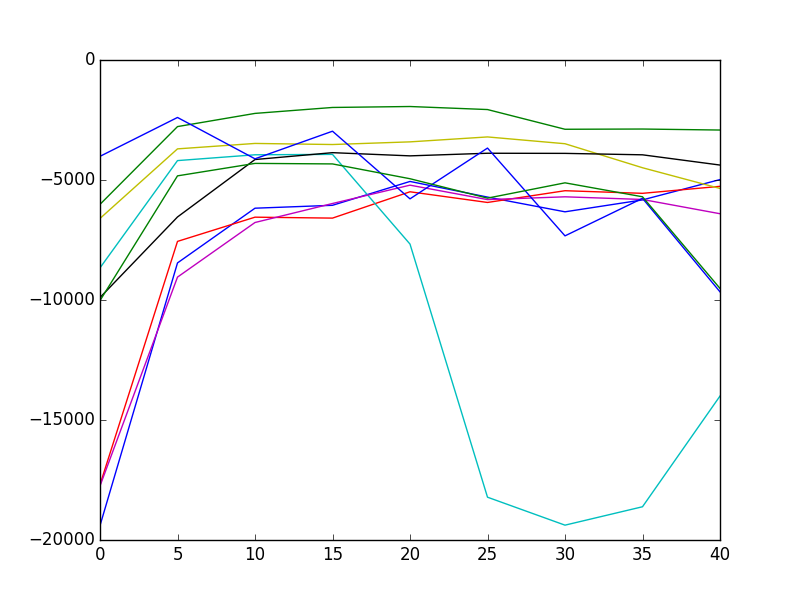
\includegraphics[width=0.5\textwidth]{figure_1}
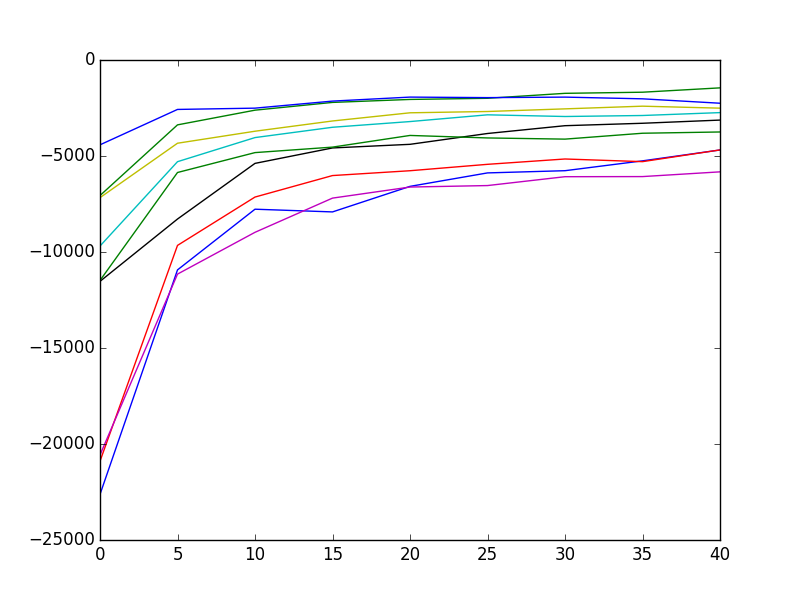
\includegraphics[width=0.5\textwidth]{figure_2}  
\begin{footnotesize}
Left: Full matrix. Right: Diagonal matrix.\\
9 Lines in different colors are 9 states(user mood). 
\end{footnotesize}
\end{figure}

The generative graphic model of HMM is trivially to describe. Each hidden state is the mood of a specific user, hidden nodes directed as time(date) sequence. Observation is 10 dimensional multivariate variable on that date. 

Here I found out the date is not continuous, so there are unobserved data between dates. To simplify the model, I assume dates of each user is continuous. However, this assumption may make big bias of hidden markov model. Since the basic assumption of markov model is the dependence of current state and the immediate previous state. In the  case of our dataset, most of the hidden variables should be independent! I still assume the date is continuous for each user, that might be one reason why the model does not perform well.

Another problem is most of the cases, the data of each user is less than 10. So training one user and test another will cause overfitting problem. So I use a different way to train the HMM model.

1, Random init Transition Matrix A, use gaussian 10 mixtures to model dataset and init means, weights and covariance. init initial state by counting state rate of whole dataset

2, Use initial paraments for training the first user. Apply EM(expectation-modification) algorithm devised by Baum-Welch to estimate weight, means, covariance, A. 

3, Use the paramenters from previous user as initial parameters to train new user.

As for testing, I usally choose half of training size users. And applied viterbi to decode state sequence. Then I evaluate the correct rate.

\section{Experiment}

Result list in Table 2.
\begin{table}
\begin{center}
\caption{Correct rate}
\scalebox{0.7}{
\begin{tabular}{|c|c|c|c|c|c|c|c|} 
\hline
Exp&diff 0 &diff 1 &diff 2  &diff 3  &diff 4 &users number &data number  \\
\hline
Training &0.39873418  &0.62025316  &0.73417722  &0.79113924  &0.86708861 &10 &158  \\
\hline
Testing &0.09090909  &0.36363636  &0.45454545  &0.72727273  &0.81818182 &5 &33  \\
\hline

 \end{tabular}
 }
 \begin{footnotesize}
diff x means $|$predict mood - target mood$|$ = x 
\end{footnotesize}
\end{center}
\end{table}

\section{Future Work}
1 Tried Possion to some features of dataset
2 Tried using structure learning for model the directed graph of each feature. It is apparently some features have dependency.
3 Dealing with the gaps of dates for each user

   

\end{document}